\documentclass[12pt]{beamer}
\usepackage[utf8]{inputenc}
\usepackage{graphicx}
\usepackage{booktabs} % For better table rules
\usepackage{amsmath} % For math symbols
% Choose a theme
\usepackage[T1]{fontenc}
\usepackage{lmodern}
\usetheme{Madrid}
\setbeamersize{text margin left=12mm, text margin right=12mm} 
\setbeamertemplate{frametitle}[default][left, leftskip=5mm] 
\setbeamertemplate{frametitle continuation}{\frametitle{References}}
\setbeamertemplate{bibliography item}[text] 
\setbeamertemplate{page number in head/foot}[appendixframenumber]
\setlength{\parskip}{5pt}
\let\oldbib\bibentry
\graphicspath{{gfx/}}
\usepackage{multicol}
\usepackage{multirow}
\usepackage{xcolor}
%\usepackage{array}
\usetheme{Madrid}  

\title[ KNUST]{\textbf{\small{Decoding Student Retention and Churn of Vodafone (Telecel) in KNUST: A Survival Analysis Approach}}}
%\subtitle{Write the subtitle}

\author[BSc. Actuarial Science]{
{\footnotesize{
Musah Faridu Oubda (4325620)\\ Kassim Asana     (4323020)\\ Sarpong Linda    (4330720) \\ Torsi Edmond Collins (4331420) \\ Asiamah Ezekiel (4316720)  }} \\[4mm] 
\includegraphics[scale=0.1]{logo.png} \\Supervisor By: S. Addai-Henne}
\institute
[COS]{ Kwame Nkrumah University Of Science And Technology, KNUST \\ Kumasi, Ghana} 

\date[\tiny \today]{\scriptsize \today}

%\titlegraphic{
\includegraphics[scale=0.08]{logo}}
\logo{
\includegraphics[scale=0.04]{logo.png}}

\setbeamercovered{transparent}
\setbeamertemplate{navigation symbols}{}


\begin{document}
	% Title page
	\begin{frame}
		\titlepage
	\end{frame}
	
	% Table of contents
	\begin{frame}{TABLE OF CONTENTS}
		\tableofcontents
	\end{frame}
		
	\begin{frame}
 	\section{BACKGROUND OF STUDY}
		\frametitle{BACKGROUND OF STUDY}
  		\begin{flushleft}

		\begin{itemize}
			\item 	The telecommunication industry is a very competitive market which makes acquiring and retaining new customers challenging.
   \vspace{0.3cm}

               \item Customer churn is the loss of clients or customers \cite{sterne2008}. They include both voluntary and involuntary churn.
               \vspace{0.3cm}
               \item   Retention is the practices and strategies a company uses to keep its existing customers.

   \end{itemize}
   		\end{flushleft}

    \end{frame}
	
	\begin{frame}
 		\section{PROBLEM STATEMENT}

		\frametitle{PROBLEM STATEMENT}
  \begin{itemize}
      \item There is a lack of understanding about the factors driving student churn and retention thus making it difficult to develop effective strategies to address this issue \cite{kapur2018}.
       % Despite the partnership with KNUST to provide mobile services to students, churn still persists.
		
  \end{itemize}
     
	\end{frame}
	
\begin{frame}
%\begin{center}
    \section{RESEARCH OBJECTIVES}

    \frametitle{RESEARCH OBJECTIVES}
    \begin{itemize}
        \item To estimate churn rate at various levels.
        \vspace{0.3cm}
        \item To determine covariates that affect the churn rate.
                \vspace{0.3cm}

        \item To identify strategies to improve retention rate and reduce churn.
                \vspace{0.3cm}

    \end{itemize}
    
    %\vfill
   % \begin{flushright}
   %     
\includegraphics[width=0.05\textwidth]{logo.png}
    %\end{flushright}
   % \end{center}

\end{frame}

    
 %   \begin{frame}
    	%	\section{SIGNIFICANCE}

	%	\frametitle{SIGNIFICANCE}
            %\begin{itemize}
%The study will pinpoint factors driving student churn from Vodafone, helping KNUST develop strategies to boost retention, improve telecom services, and strengthen the KNUST-Telecel partnership by better meeting students' needs.             %\end{itemize}
%    \end{frame}
    
	
	
	
	\begin{frame}
 	\section{METHODOLOGY}

		\frametitle{METHODOLOGY}
		\begin{itemize}
			\item \textbf{Data collection}\\
The data used for the study was obtained through simple random sampling of level 400 students in College of Science. The dataset consisted of  338 observations and 14 variables. 
	
   		\vspace{0.3cm}

			\item \textbf{Data pre-processing}\\
The data was then encoded to transform all categorical data into a numerical format to facilitate the analysis.

   	\end{itemize}
    \end{frame}


\begin{frame}

		\frametitle{METHODOLOGY CONT'D}
    \framesubtitle{Fundamental Concept of Survival Analysis}  
		\begin{itemize}
            \item  \textbf{Survival Function $S(t)$ }\\
This is a general framework in survival analysis to determine the probability that a person survives longer than some specified time.
\begin{equation}\scriptsize
    S(t) = Pr{(T \geq t)}
\end{equation}
    \item \textbf{Hazard Function $h(t)$}\\
   The hazard function denotes the instantaneous rate of failure at time $t$, given that the subject has survived up to time $(t)$. 
 \begin{equation} \scriptsize
h(t) = \lim_{\Delta t \to 0} \frac{P(t \le T < t + \Delta t \mid T \geq t)}{\Delta t}
\end{equation}
\scriptsize $$h\left(t\right)\geq0$$

   	\end{itemize}

    \end{frame}
 

\begin{frame}


		\frametitle{METHODOLOGY CONT'D}
      \framesubtitle{Survival Models}  

		\begin{itemize}
            \item  \textbf{Kaplan Meier }\\
It is to analyze the survival probability of the time until an event occurs.
\begin{equation} \scriptsize
S\left(t\right)=\prod_{i:t_i\le t}\left(1-\frac{d_i}{n_i}\right)
\end{equation}
    \item \textbf{Cox Proportional (Cox PH) Hazard Model}\\
  It is used to study the impact of different covariates on survival time.
\begin{equation} \scriptsize
h\left(t \mid x\right) = h_0(t) \exp(\beta_1 x_1 + \beta_2 x_2 + \cdots + \beta_p x_p)
\end{equation}

    \item \textbf{Accelerated Failure Time (AFT)}\\
 It is used to analyze the time until an event occurs by assuming a specific distribution for survival time. 
\begin{equation} \scriptsize
\lambda(x) = \exp(b_0 + \sum_{i=1}^{n}{b_i x_i})
\end{equation}


   	\end{itemize}

    \end{frame}
 

\begin{frame}
    \frametitle{METHODOLOGY CONT'D}
        \framesubtitle{Model Comparison}  

    \begin{itemize}
        \item \textbf{Concordance Index (C-Index)}\\
        It is used to evaluate the predictive accuracy of a survival model. 
        \begin{equation} \scriptsize
        C=\frac{Number\ of\ Concordant\ Pairs}{Number\ of\ Concordant\ Pairs\ +Number\ of\ Discordant\ Pairs}
        \end{equation}
        \item \textbf{Information Criteria and Loglikelihood}\\
        It is used to evaluate how well a survival model fits the dataset.
        \begin{table}[H]
        \centering
        \begin{tabular}{|c|c|c|}
        \hline
         \textbf{AIC} & \textbf{HQIC} & \textbf{BIC} \\
        \hline
         \(2k - 2\ln(L)\) & \(-2\ln(L) + 2k\ln(\ln(n))\) & \(k\ln(n) - 2\ln(L)\) \\
        \hline
        \end{tabular}
        \caption{Information Criteria Formulas}
        \label{table:info_criteria}
        \end{table}
    \end{itemize}
\end{frame}
	%\begin{frame}
	%	\frametitle{METHODOLOGY}
%\begin{figure}
    %\centering
     % \caption{Methodology}
   % 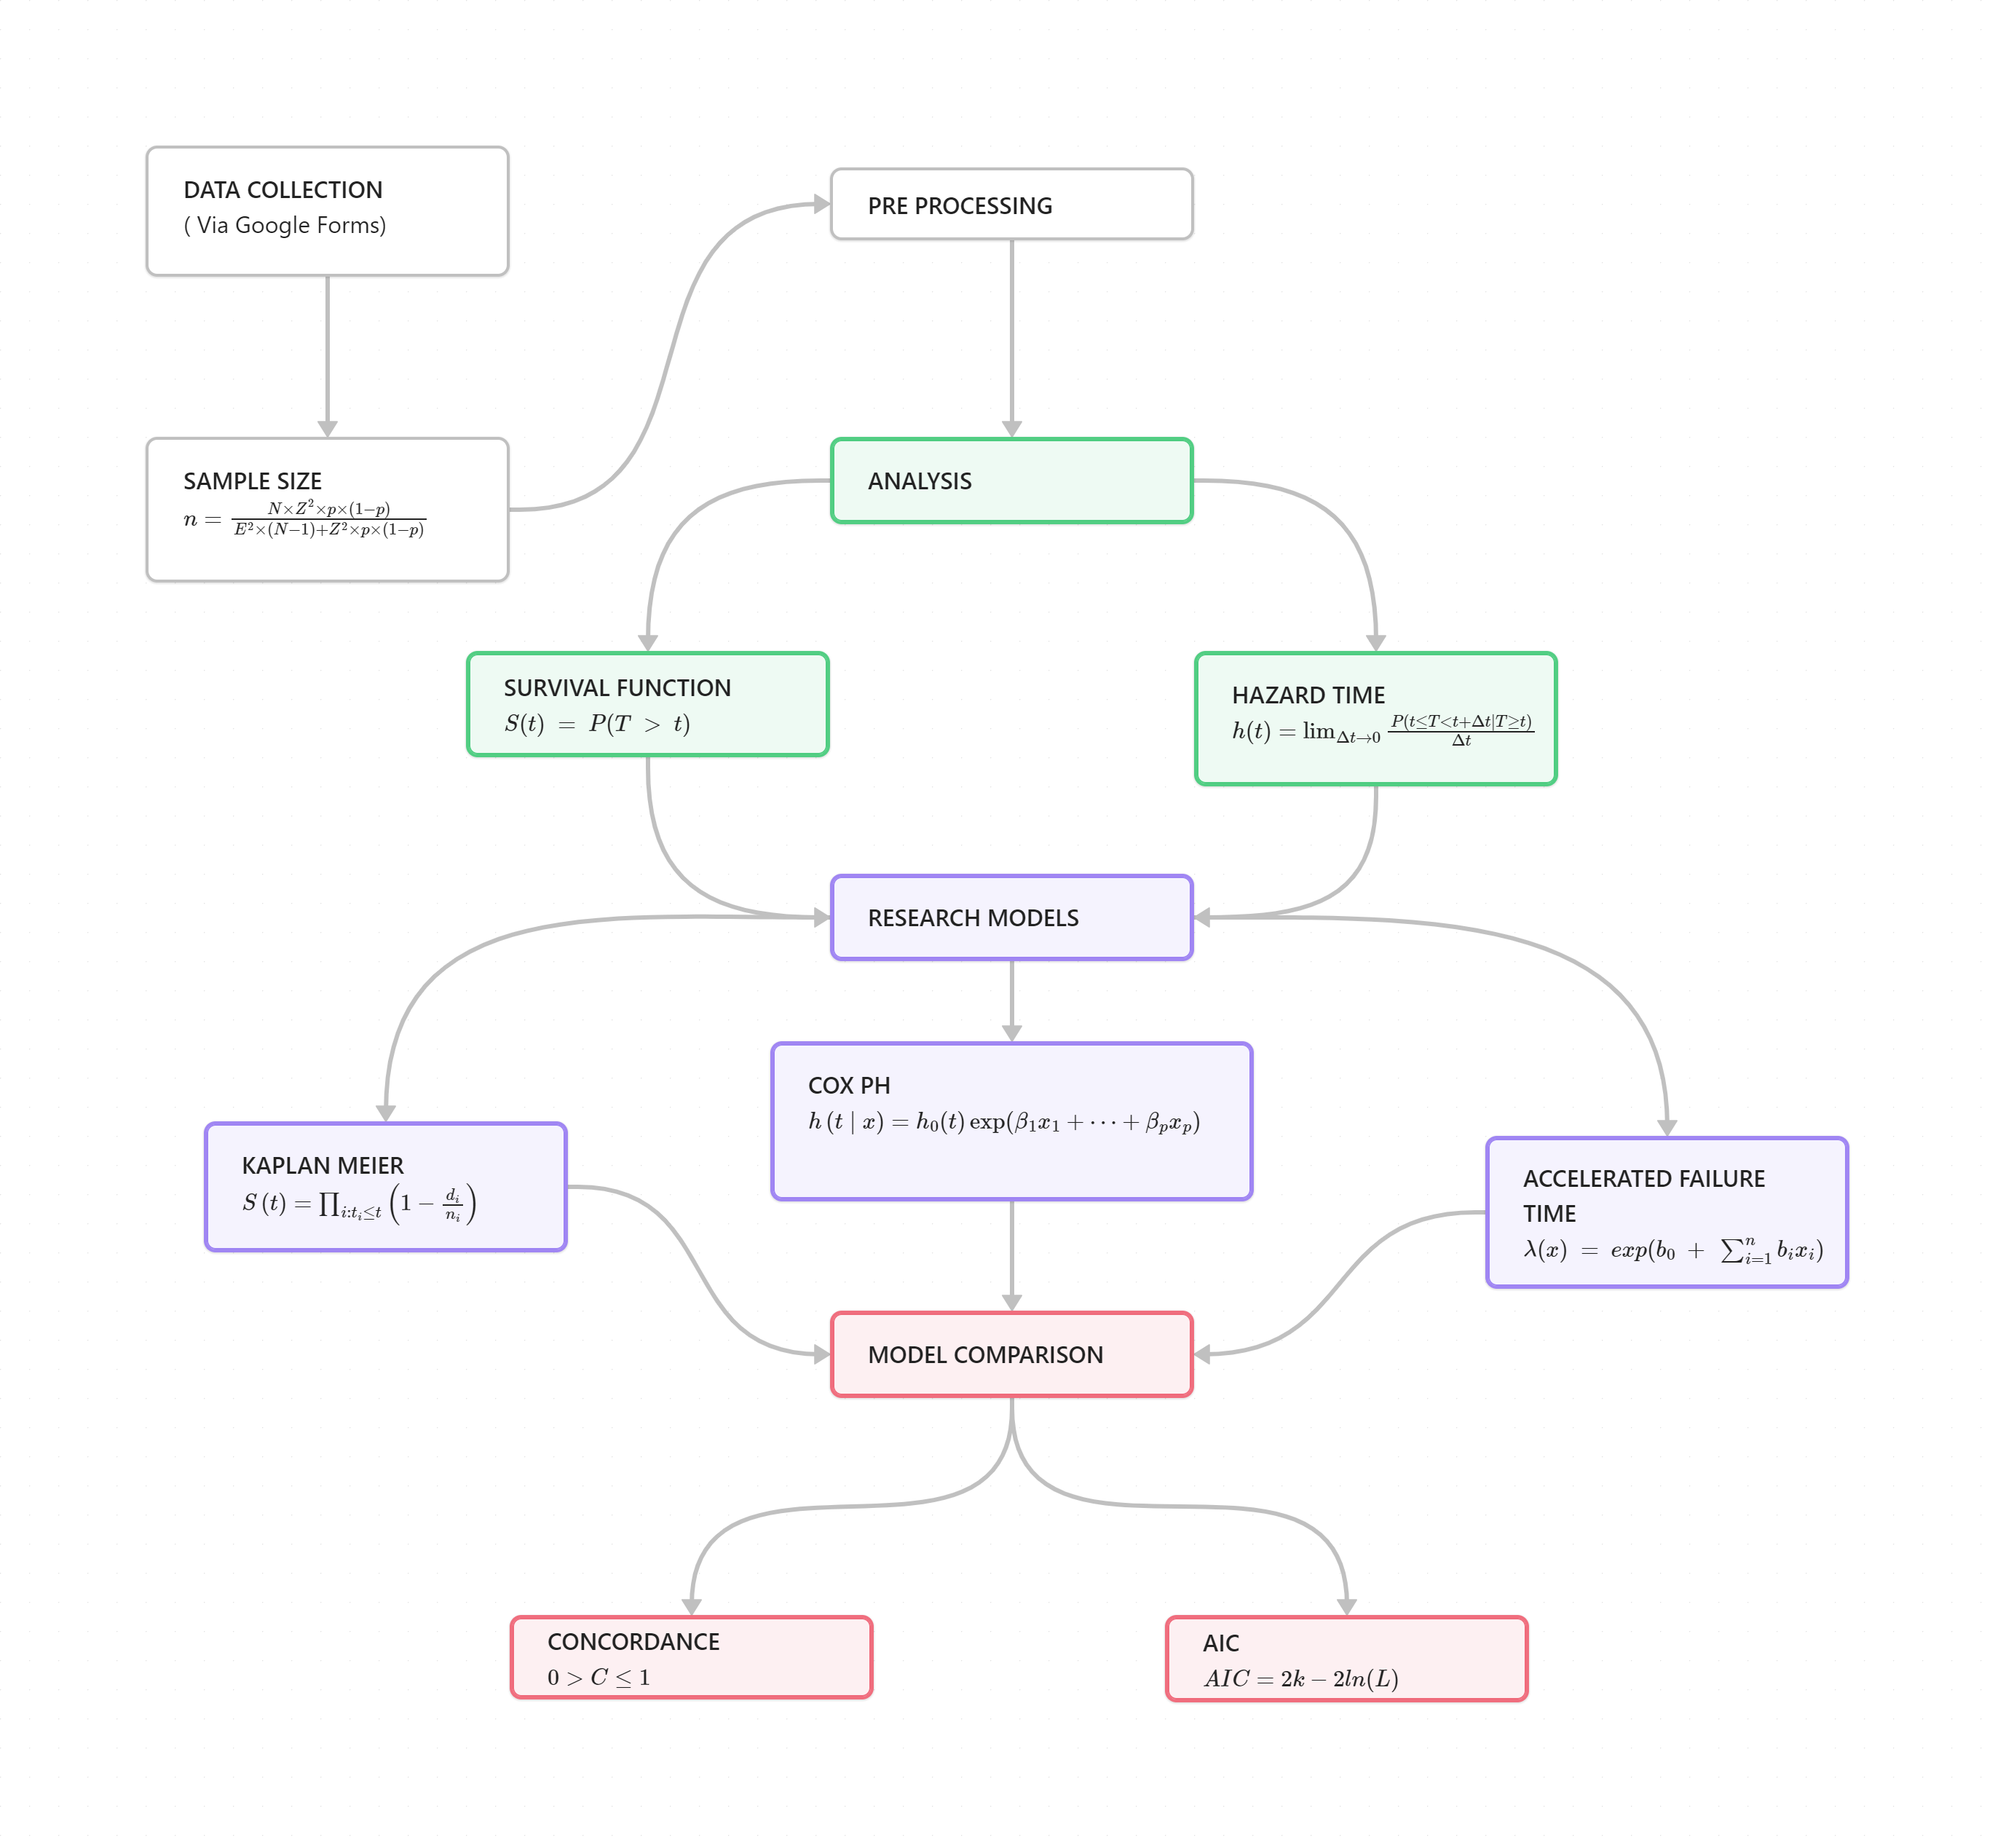
\includegraphics[width=0.65\linewidth]{Presentation/Methodology.png}
  
   % \label{fig:enter-label}
%\end{figure}

	%\end{frame}
	
	\begin{frame}
  	\section{ANALYSIS AND FINDINGS}

    \frametitle{ANALAYSIS AND FINDINGS}
    \framesubtitle{Descriptive Analysis}
    \begin{block}{}
        Out of the 338 students, 79 were recorded to have churned over the years while 259 had not churned.
    \end{block}

\begin{figure}[H]
    \centering
    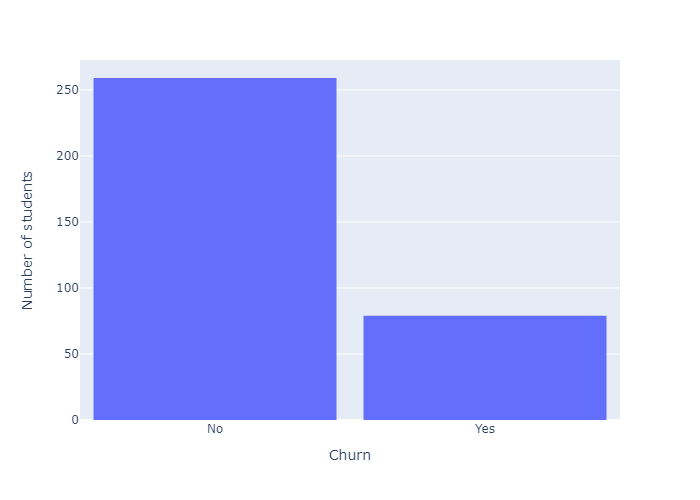
\includegraphics[width=0.68\linewidth, height=0.5\textheight]{Figure 4/distribution.png}
    \caption{Descriptive Analysis of Churn Data}
    \label{fig:enter-label}
\end{figure}


\end{frame}

 
\begin{frame}

    \frametitle{ANALAYSIS AND FINDINGS CONT'D}
    
    \begin{block}{Kaplan Meier}
        The Kaplan-Meier survival analysis below estimates the survival probability at the end of various academic years.
    \end{block}
    
   % Add some vertical space between the block and the content
    
   \begin{table}[H]
\centering
\begin{tabular}{ccc}
\hline
\textbf{Event Time} & \textbf{Number of Events} & \textbf{Survival Probability} \\
\hline
0& 0  & 1.000000 \\
1& 25 & 0.926036 \\
2& 22 & 0.860947 \\
3& 32 & 0.766272 \\ \hline
\end{tabular}
\caption{Survival Analysis Summary}
\label{Kaplan Meier Table}
\end{table}


\end{frame}


\begin{frame}
    \frametitle{ANALAYSIS AND FINDINGS CONT'D}
     \framesubtitle{Kaplan Meier Curve}

    
		\begin{figure}[H]
			\centering
			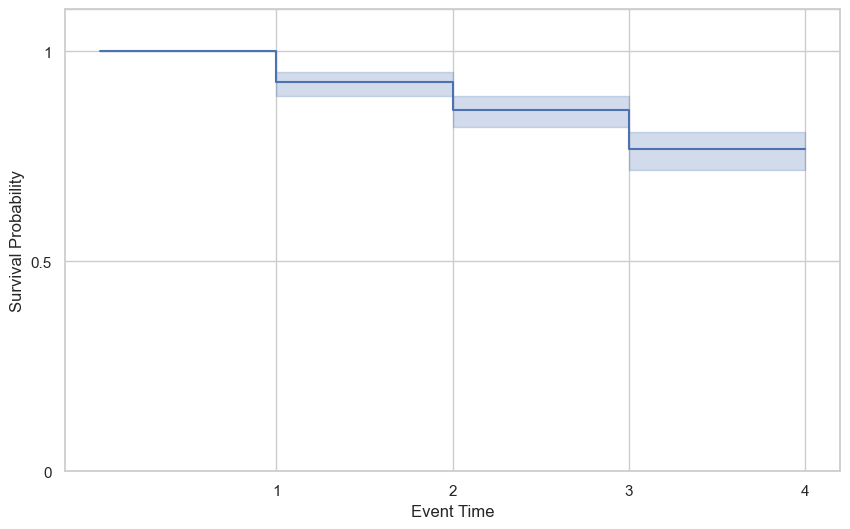
\includegraphics[width=0.9\textwidth]{Figure 4/4.1.png}
			\hfill
			\caption{Kaplan Meier Curve}
			
		\end{figure}

\end{frame}

	\begin{frame}
     \frametitle{ANALAYSIS AND FINDINGS CONT'D}

 		\framesubtitle{Accelerated Failure Time}
            \begin{block}{Selection of parametric distribution}
The LogNormal model is the best based on AIC and BIC values, showing the best fit among the distributions.
\end{block}

  \begin{table}[H]
        \centering
        \begin{tabular}{lccc}
            \hline
            Model & AIC & BIC & Hannan-Quinn \\
            \hline
            Weibull & 316.43 & 300.08 & 306.67 \\
            \textbf{LogNormal} & \textbf{305.81} & \textbf{289.45} & \textbf{306.67} \\
            LogLogistic & 307.51 & 291.16 & 306.67 \\
            \hline
        \end{tabular}
        \caption{Information Criteria on AFT Models}
        \label{tab:model_comparison}
    \end{table}

    \end{frame}
	
	\begin{frame}
    \frametitle{ANALYSIS AND FINDINGS CONT'D}
        \framesubtitle{Comparison between Cox PH and AFT}  

    \begin{table}[H]
    \centering
    \scriptsize
    \setlength{\tabcolsep}{3pt} % Reduce column separation
        \scriptsize{* indicates significant covariate.}

    \begin{tabular}{lcc|cc}
    \toprule
    Variable & \multicolumn{2}{c}{Cox PH Model} & \multicolumn{2}{c}{Lognormal Model} \\
    \cmidrule(lr){2-3} \cmidrule(lr){4-5}
     &   \scriptsize{$\beta$}& \scriptsize{P-values}& \scriptsize{$\beta$}& \scriptsize{P-values}\\
    \midrule
    Gender & 0.33 & 0.24 & 0.032 & 0.785 \\
    Residence & 0.32 & 0.25 & -0.146 & 0.239 \\
    Usage Freq. & -0.08 & 0.27 & -0.002 & 0.940 \\
    Voice Calls & -0.57 & 0.08 & 0.132 & 0.329 \\
    Mobile Data & 0.32 & 0.48 & -0.287 & 0.165 \\
    \textbf{SMS}& 0.48 & 0.06 & -0.228 & 0.036*\\
    Data Exhaust. & -0.20 & 0.61 & 0.102 & 0.493 \\
    Multiple Networks& -0.13 & 0.78 & -0.104 & 0.607 \\
    \textbf{Poor Network}& 2.60 & <0.005* & -1.041 & <0.0005*\\
    \textbf{Customer Service}& -1.40 & <0.005* & 0.809 & <0.0005*\\
    \textbf{High Costs}& -1.13 & <0.005* & 0.515 & <0.0005*\\
    \textbf{Monthly Data}& 0.21 & 0.02* & -0.069 & 0.113 \\
    \midrule
    Intercept $\mu$ & -- & -- & 1.626 & <0.0005 \\
    Intercept $\sigma$ & -- & -- & -0.616 & <0.0005 \\
    \bottomrule
    \end{tabular}
    \scriptsize{\caption{Cox PH and LogNormal Models}}
    
    \label{tab:combined_model_results}
    \end{table}
    \scriptsize{* indicates significant covariate.}
    \end{frame}

	
	\begin{frame}
		\frametitle{ANALYSIS AND FINDINGS}
        \framesubtitle{Selection of distribution}
      \framesubtitle{Cox Proportional Hazard Plot}  

		\begin{figure}[H]
			\centering
			\begin{minipage}{0.8\textwidth}
				\centering
				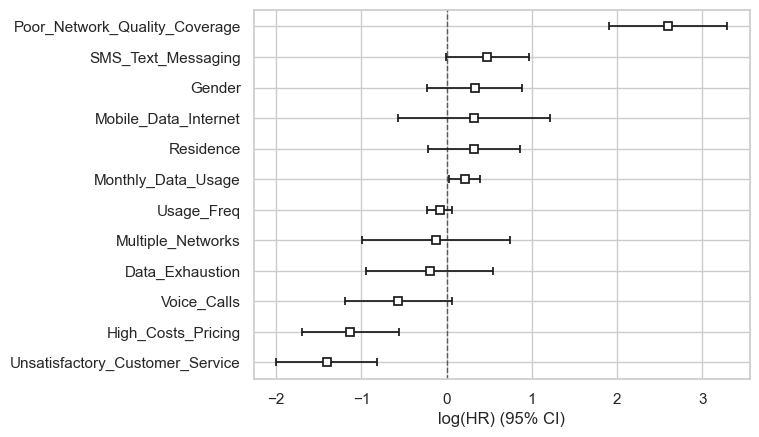
\includegraphics[width=\textwidth]{Figure 4/4.2.png}
				\caption{Cox PH Forest Plot}
				\label{Figure 3}
			\end{minipage}
		
		\end{figure}
A positive covariate indicates an increase in churn rate while the negative covariate indicates a decrease in churn rate.
 \end{frame}
 
	\begin{frame}
		\frametitle{ANALYSIS AND FINDINGS CONT'D}
      \framesubtitle{Accelerated Failure Time Plot}  

		\begin{figure}[H]
			\centering
			\begin{minipage}{0.8\textwidth}
				\centering
				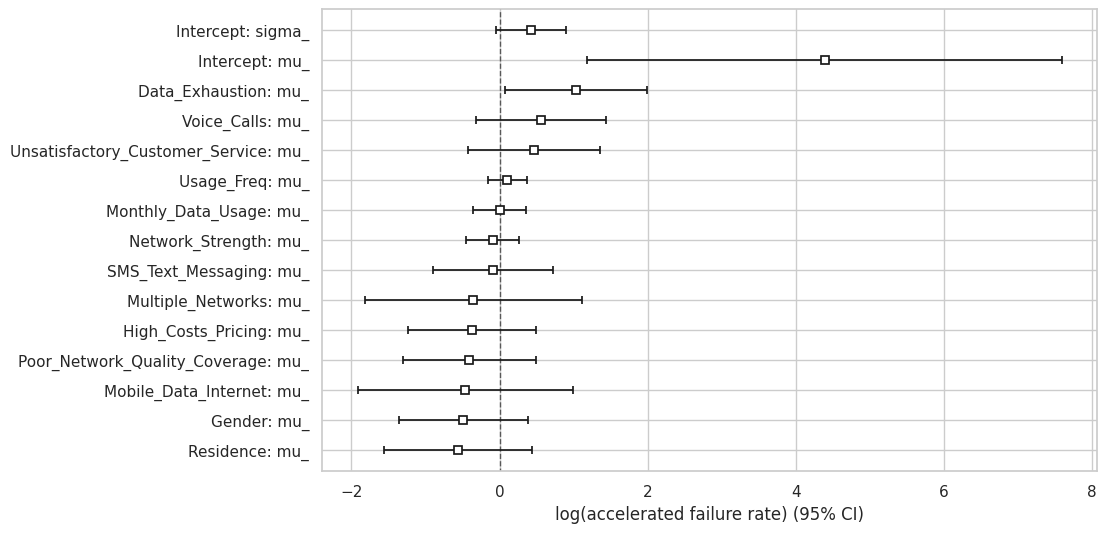
\includegraphics[width=\textwidth]{Figure 4/4.4.png}
				\caption{LogNormal Forest Plot}
				\label{Figure 4}
				
			\end{minipage}
        \end{figure}
A positive covariate indicates a decrease in the time to event while the negative covariate indicates an increase in the time to event.	
 \end{frame}
  

	\begin{frame}
		\frametitle{MODEL COMPARISON}
		%Table here
		\begin{table}[H]
			\centering
			\begin{tabular}{lcc}
				\toprule
				\textbf{Model} & \textbf{Concordance} & \textbf{Loglikelihood}\\
				\midrule
				LogNormal& 0.958& 	290.678 \\
				Cox PH & 0.96& 	266.68\\
				\bottomrule
			\end{tabular}
			\caption{Model Concordance and Loglikelihood values}
			\label{Table 2}
			
		\end{table}
		
	\end{frame}
	
	
	\begin{frame}
 	\section{CONCLUSION}

		\frametitle{CONCLUSION}
		\begin{itemize}
			\item The research indicates that the Cox PH model provides the best predictions for the data, while the LogNormal model offers the best fit. 
            \vspace{0.3cm}

           \item Poor Network, Customer Service, High Costs, Monthly Data, and SMS are the most significant covariates in the study.
           \vspace{0.3cm}
           
			\item Poor Network Quality tends to increase both the churn rate and time to churn the most.
            \vspace{0.3cm}
			\item Students tend to churn most in their 3rd year.
		\end{itemize}
	\end{frame}
 
	
	\begin{frame}
		\frametitle{RECOMMENDATIONS}
  \section{RECOMMENDATIONS}
		\begin{itemize}


			\item Enhance the quality and reliability of network coverage across KNUST to reduce churn rates.
\vspace{0.3cm}

			\item Establishment of avenues and platforms to address students' concerns more effectively.
    
    \end{itemize}	
 \end{frame}
	
	\begin{frame}
 \section{REFERENCES}
		\frametitle{REFERENCES}
 \bibliography{references_presentation}
 \bibliographystyle{apalike}
 \end{frame}
	
	\begin{frame}
\frametitle{\phantom{ }}  		
  \centering\Large{\textbf{ THANK YOU}}
		
		
		
	\end{frame}
\end{document}
